\chapter{Studi Literatur}

\section{Pengantar Jaringan Komputer}
Menurut \textcite{forouzan2012}, jaringan komputer merupakan sebuah keterhubungan dari beberapa perangkat yang dapat melakukan komunikasi satu sama lain. Perangkat yang dapat terlibat pada jaringan komputer ini sapat berupa \emph{host} seperti komputer, laptop, dan gawai lainnya. Selain itu, perangkat pada definisi di atas dapat berupa perangkat penghubung. Beberapa contoh dari perangkat penghubung adalah \emph{router}, \emph{switch}, dan \emph{modem}.

Terdapat empat buah syarat sebuah sistem dapat dikatakan sebagai jaringan komputer menurut \textcite{pratama2015}. Syarat-syarat yang perlu dipenuhi adalah sebagai berikut:
\begin{enumerate}
  \item Dalam sebuah sistem, setidaknya terdapat dua buah perangkat yang terhubung. Perangkat tersebut dapat terhubung melalui sarana kabel (\emph{wired}) ataupun sarana nirkabel (\emph{wireless}).
  \item Pada sistem ini, terdapat pengguna yang melakukan interaksi dengan pengguna lainnya. Pengguna ini dapat berupa penyedia layanan atau seseorang yang hendak melakukan komunikasi melewati jaringan komputer.
  \item Pada sistem ini, terdapat data yang dipertukarkan di dalamnya. Jenis data yang dipertukarkan dapat berupa pesan teks ataupun pesan biner.
  \item Terdapat sebuah sumber daya yang digunakan secara bersama-sama. Sumber daya ini dapat berupa perangkat keras ataupun perangkat lunak.
\end{enumerate}

\subsection{Pemodelan Jaringan TCP/IP}
Menurut \textcite{odom2022}, pemodelan jaringan merupakan kumpulan dari berbagai dokumen yang menjelaskan sebuah fungsionalitas dalam sebuah jaringan. Dokumen-dokumen ini akan mendefinisikan hal-hal yang terjadi pada jaringan komputer saat bekerja. Beberapa dokumen bisa saja menjelaskan sebuah protokol jaringan, yaitu kumpulan aturan yang perlu dipenuhi saat sebuah perangkat melakukan komunikasi pada jaringan komputer.

Pemodelan jaringan TCP/IP merupakan pemodelan terbaru yang memperbaiki kekurangan yang ada pada pemodelan \emph{layer} OSI (\cite{forouzan2012}). Selain itu, munculnya pemodelan jaringan TCP/IP dikarenakan pemodelan OSI \emph{layer} sudah tidak relevan dalam pemodelan jaringan. Faktanya, Pemodelan jaringan OSI pada saat ini sudah tidak ada lagi (\cite{odom2022}), tetapi beberapa protokol pada pemodelan TCP/IP masih merujuk pada protokol asli yang ada pada \emph{layer} OSI.

Pemodelan jaringan TCP/IP dibagi menjadi lima lapisan. Menurut \textcite{forouzan2012}, lapisan tersebut di antaranya sebagai berikut:

\begin{enumerate}
  \item \emph{Application Layer}: Lapisan ini menjelaskan spesifikasi aplikasi agar dapat berkomunikasi dalam jaringan komputer. Lapisan ini berfungsi sebagai antar muka antara aplikasi dengan jaringan. Beberapa contoh protokol yang berada pada lapisan ini adalah HTTP, FTP, dan SSH.
  \item \emph{Transport Layer}: Lapisan ini menjelaskan cara untuk memecah paket data menjadi unit-unit data yang lebih kecil (yang disebut sebagai \emph{segment}). Selain itu, lapisan ini juga berfungsi untuk memberikan penomoran setiap unit paket data sehingga data yang didapatkan akan terurut saat diberikan kepada aplikasi. Beberapa contoh protokol yang bekerja pada tingkatan ini adalah TCP dan UDP.
  \item \emph{Network Layer}: Lapisan ini menjelaskan bagaimana sebuah paket data dalam melakukan proses \emph{routing} untuk mencapai tujuan. Pada lapisan ini, dikenal sebuah sistem pengalamatan yang disebut dengan IP (\emph{Internet Protocol}) yang terstandarisasi secara internasional.
  \item \emph{Data Link Layer}: Lapisan ini bertugas untuk mengkontrol data, mengontrol kesalahan pada data saat pengiriman, serta pengalamatan fisik. Pada lapisan ini juga, didefinisikan cara untuk mengontrol aliran paket (\emph{Flow Control}) pada sebuah jaringan.
  \item \emph{Physical Layer}: Lapisan ini bertugas untuk menjelaskan perangkat keras dari sebuah jaringan komputer. Selain itu, lapisna ini juga bertugas untuk membantu proses persinyalan dan sinkronisasi bit data.
\end{enumerate}

\subsection{Protokol TCP}
Menurut \textcite{pratama2015}, Protokol TCP merupakan protokol jaringan pada lapisan \emph{transport} yang bersifat dapat diandalkan (\emph{reliable}) dan berbasis koneksi (\emph{connection oriented}). TCP memiliki sifat keandalan dikarenakan adanya proses pemeriksaan \emph{segment} yang dikirimkan ke komputer tujuan. Hal ini terlihat adanya pesan berupa konfirmasi dari penerima. Selain itu, TCP merupakan protokol berbasis koneksi. Hal ini dikarenakan saat sebelum melakukan pengiriman data, protokol ini mengharuskan untuk membentuk koneksi jaringan komputer terlebih dahulu. 

Menurut \textcite{peterson2011}, Terdapat beberapa layanan yang disediakan oleh protokol TCP. Layanan-layanan tersebut memberikan jaminan pada aplikasi bahwa data yang diterima dapat dipastikan terurut dan tidak hilang. Beberapa layanan yang disediakan di antaranya adalah sebagai berikut.

% Semuanya dari peterson2011 %
\begin{enumerate}
  \item Keandalan (\emph{Reliability}): Pada protokol TCP, data yang dikirimkan terjamin keterurutan saat diterima oleh penerima. Selain itu, proses pengiriman pada TCP bersifat \emph{full-duplex}. Hal ini berarti proses pengiriman data dapat dilakukan dua arah secara bersama-sama. Pada protokol ini juga, terdapat mekanisme kontrol aliran data. Hal ini memungkinkan untuk pengirim atau penerima menentukan jumlah data yang dikirimkan dalam satu waktu.
  \item Berbasis koneksi (\emph{Connection Oriented}): Protokol TCP mengharuskan pembuatan koneksi pada saat sebelum pengiriman data. Proses pembentukan koneksi ini perlu untuk membangun koneksi tidak hanya pada pengirim dan penerima, tetapi juga pada seluruh perangkat jaringan yang terlibat. Selain itu, protokol TCP juga mengharuskan pemutusan koneksi saat komunikasi berakhir. 
  \item Layanan pengiriman alir: Pada TCP, aplikasi memungkinkan untuk mengirimkan \emph{byte-byte} data menuju aliran jaringan. TCP akan menentukan seberapa banyak data yang akan dikirimkan menuju penerima.
\end{enumerate}

Menurut \textcite{pratama2015}, terdapat tiga tahap koneksi yang perlu dilakukan saat mengirimkan data. Ketiga tahap tersebut adalah pembentukan koneksi, pengiriman data, serta terminasi koneksi. Ketiga tahap ini perlu dilakukan dikarenakan sifat dari protokol TCP yaitu berbasiskan koneksi.

Tahap pertama yang perlu dilakukan dalam mengirim data melalui TCP adalah pembentukan koneksi. Proses pembentukan koneksi dilakukan dengan menggunakan \emph{three way handshake}. Menurut \textcite{peterson2011}, \emph{server} membentuk koneksi pasif dengan \emph{client}. Selanjutnya, \emph{client} mengirimkan \emph{segment} ACK menuju server. Setelah server menerima \emph{segment} ACK, server akan mengirimkan \emph{segment} SYN+ACK. Setelah itu, \emph{client} mengirimkan \emph{segment} ACK menuju \emph{server}. Setelah semua proses ini terjadi, koneksi antar \emph{client} dan \emph{server} telah terjalin. Proses ini dapat digambarkan pada \ref{fig:tcp.open}. 

\begin{figure}[!h]
  \centering
  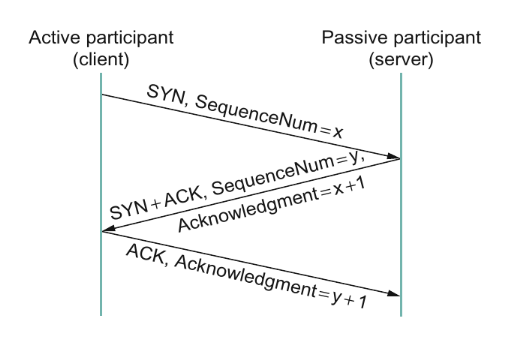
\includegraphics[width=\textwidth]{chapters/res/chapter-2/img/tcp.open.png}
  \caption{Proses Pembukaan Koneksi TCP} \label{fig:tcp.open}
  Sumber: \textcite{peterson2011}
\end{figure}

Saat koneksi telah terjalin, pengiriman data sudah dapat dilakukan. Proses transfer data dilakukan dengan mengirimkan \emph{segment} data menuju penerima. Saat menerima data, penerima harus mengirimkan \emph{segment} ACK menuju pengirim. Apabila terjadi kegagalan transmisi, setiap \emph{segment} yang hilang harus ditransmisikan ulang.

Menurut \textcite{peterson2011}, setiap \emph{segment} yang dikirimkan diharapkan selalu penuh. Hal ini mencegah terjadi permasalahan \emph{silly window syndrome}. Oleh karena itu, pengiriman dapat diatur oleh algoritma nagle. Terdapat sebuah parameter untuk menentukan besar maksimum data yang dikirimkan yaitu nilai \emph{maximum segment size} (MSS).

Pada saat pengiriman data, terdapat juga sebuah nilai $Timeout$ yang menentukan apakah proses pengiriman \emph{segment} perlu diulang. Nilai ini dapat diturunkan melalui nilai estimasi \emph{round time trip} (RTT) dari sebuah data. Menurut \textcite{peterson2011}, Nilai estimasi RTT ditentukan dengan persamaan \ref{eq:tcp.rtt}.

\begin{equation}
  \label{eq:tcp.rtt}
  EstimatedRTT_{i+1} = \alpha \times EstimatedRTT_i + (1 - \alpha) \times SampleRTT_i
\end{equation}

Nilai $SampleRTT_i$ diambil melalui data yang telah diterima pada saat ke-$i$. Nilai ini menyatakan waktu dimulainya sebuah \emph{segment} ditransmisi hingga diterimanya \emph{segment} ACK. Nilai $\alpha$ digunakan untuk membuat nilai $EstimatedRTT$ menjadi lebih \emph{smooth}. Nilai $Timeout$ dapat dihitung berdasarkan persamaan \ref{eq:tcp.timeout}

\begin{equation}
  \label{eq:tcp.timeout}
  Timeout_{i} = 2 \cdot SampleRTT_i
\end{equation}

Saat mengirimkan data, pengirim perlu menunggu ACK hingga batas $timeout$. Apabila telah terjadi timeout, pengirim perlu mengirimkan ulang data mereka menuju penerima. Semua proses pada tahap pengiriman ini perlu dilakukan hingga semua data berhasil dikirimkan.

Pada fase terakhir, koneksi antara \emph{client} dan \emph{server} perlu ditutup. Hal ini perlu dilakukan dengan \emph{client} melakukan proses \emph{active close}. Pada tahap \emph{active close}, \emph{client} mengirimkan pesan FIN. Setelah itu, \emph{server} mengirimkan pesan FIN+ACK. Setelah menerima pesan dari \emph{server}, \emph{client} perlu mengirimkan ACK. Setelah itu, koneksi antara \emph{server} dan \emph{client} telah tertutup.

\section{Pengantar Kriptografi}
Menurut \textcite{schneier1996}, Kriptografi merupakan ilmu pengetahuan dan seni yang berujuan untuk menjaga sebuah pesan tetap aman. Menurut \textcite{anderson2008}, Kriptografi dianggap sebagai pintu para pengembang keamanan untuk bertemu dengan ilmu matematika. Hal ini dapat terlihat bahwa banyak sekali algoritma kriptografi yang terkait dengan konsep matematika. Kriptografi dianggap juga sebagai seni. Menurut \textcite{munir2019}, hal ini dikarenakan dari pandangan sejarah berkembangnya kriptografi. Kriptografi ini terbentuk dikarenakan adanya keinginan untuk merahasiakan sebuah pesan. Tentu saja, setiap orang memiliki ciri khas serta caranya tersendiri untuk menyandikan sebuah pesan. Oleh karena itu, kriptografi dapat dianggap sebagai seni untuk merahasiakan sebuah pesan. 

Kriptografi pada dasarnya memiliki beberapa layanan dasar yang dapat digunakan dalam dunia keamanan. Menurut \textcite{schneier1996}, beberapa layanan yang terdapat pada kriptografi adalah sebagai berikut:
\begin{itemize}
  \item Kerahasiaan (\emph{confidentiality}) merupakan sebuah layanan yang diberikan oleh kriptografi untuk menjaga pesan agar pesan hanya dapat dimengerti oleh pihak yang memiliki otoritas. 
  \item Integritas (\emph{integrity}) merupakan layanan yang menjamin bahwa pesan yang diterima merupakan pesan yang belum pernah dilakukan modifikasi sebelumnya. Layanan ini menjamin data yang diterima sama dengan data tersebut saat pertama kali dikirim.
  \item Otentikasi (\emph{authentication}) merupakan layanan yang menjamin bahwa pesan yang diterima merupakan pesan yang dikirim oleh pengirim sesungguhnya. Hal ini terkait dengan klaim bahwa pesan yang dikirimkan tentu saja dapat dilakukan dekripsi dengan kunci yang telah disepakati.
  \item Anti penyangkalan (\emph{non-repudiation}) merupakan layanan yang menjamin bahwa pengirim tentu saja tidak akan dapat menyangkal pesan yang telah dia kirimkan.
\end{itemize} 

\section{Kriptografi Modern}
Kriptografi modern, menurut \textcite{munir2019}, merupakan kriptografi yang bekerja pada komputer digital. Pesan tidak hanya terbatas pada tulisan dan alfabet, namun pesan juga dapat berupa berbentuk apapun selama dapat diubah menjadi bentuk biner. Dalam Kriptografi modern, terdapat sebuah konsep yang disebut dengan kriptografi kunci publik, konsep fungsi \emph{hash}, serta tanda tangan digital. Hal ini merupakan konsep baru yang dapat digunakan untuk menjamin integritas serta anti penyangkalan dari pengirim pesan.

Menurut \textcite{schneier1996}, keamanan kriptografi modern tidak hanya cukup apabila merahasiakan algoritma penguncian. Hal ini dikarenakan apabila sebuah algoritma penguncian dapat dipecahkan, algoritma tersebut perlu diganti dengan yang baru. Dalam kriptografi modern, kerahasiaan yang perlu dijaga terletak pada kunci. Setiap operasi enkripsi serta dekripsi tentu saja akan melibatkan kunci ini. 

\subsection{Algoritma Kriptografi Modern}

Sebuah Algoritma modern tentu membutuhkan kunci untuk melakukan proses enkripsi dan dekripsi. Menurut \textcite{schneier1996}, algoritma kriptografi dapat dibagi menjadi dua, yaitu Kriptografi kunci simetrik dan kriptografi publik. Perbedaan dari kedua algoritma tersebut terletak pada kunci yang digunakan untuk melakukan enkripsi serta dekripsi pesan. 

Menurut \textcite{munir2019}, algoritma kunci simetri menggunakan kunci yang sama saat melakukan proses enkripsi serta dekripsi pesan. Asumsi yang diterapkan pada penggunaan algoritma ini adalah pengirim serta penerima sudah melakukan proses pembagian kunci. Skema proses enkripsi digambarkan pada gambar \ref{fig:crypto.symetric}. Beberapa contoh algoritma yang termasuk pada algoritma ini adalah \emph{Advanced Encryption Standard (AES)}, RC4, dan DES.

\begin{figure}[!h]
  \centering
  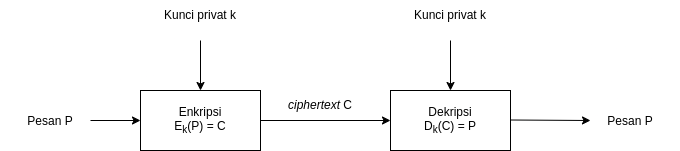
\includegraphics[width=\textwidth]{chapters/res/chapter-2/img/crypto.symetric.png}
  \caption{Visualisasi Proses Enkripsi Kriptografi Kunci Simetri} \label{fig:crypto.symetric}
  Sumber: \textcite{munir2019}
\end{figure}

Menurut \textcite{munir2019}, algoritma kunci publik (atau bisa disebut algoritma kunci nirsimetris) merupakan algoritma enkripsi yang menggunakan kunci yang berbeda pada saat melakukan proses enkripsi dan juga proses dekripsi. Pada saat melakukan komunikasi menggunakan algoritma ini, pihak yang terlibat harus memiliki satu buah kunci, yaitu kunci publik dan kunci privat. Pengirim pesan akan menggunakan kunci publik untuk mengunci pesan. Akan tetapi, penerima menggunakan kunci privat miliknya untuk membuka pesan. Dengan menggunakan algoritma ini, hanya penerima pesan yang dapat membuka pesan. Ilustrasi terkait enkripsi memanfaatkan algoritma ini terdapat pada Gambar \ref{fig:crypto.asymetric}. Beberapa contoh algoritma enkripsi kunci publik adalah RSA, \emph{Elgamal}, dan DSA.

\begin{figure}[!h]
  \centering
  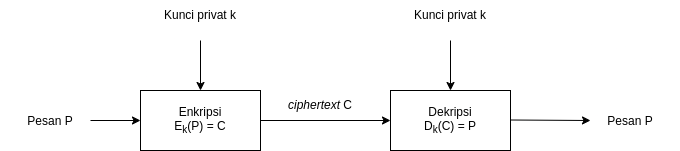
\includegraphics[width=\textwidth]{chapters/res/chapter-2/img/crypto.symetric.png}
  \caption{Visualisasi Proses Enkripsi Krpitografi Kunci Publik} 
  \label{fig:crypto.asymetric}
  Sumber: \textcite{munir2019}
\end{figure}

Menurut \textcite{munir2019}, keuntungan menggunakan kriptografi kunci publik ada dua. Keuntungan pertama adalah tidak adanya kebutuhan dalam mendistribusikan kunci rahasia. Kunci publik dapat dikirimkan melalui saluran yang tidak aman. Selain itu, keuntungan lain dari penggunaan kunci publik ini adalah jumlah pembuatan kunci dapat dikurangi. Pada saat menggunakan kriptografi kunci simetri, jumlah kunci yang harus dibuat adalah sebanyak jumlah pihak yang ingin berkomunikasi. Pada saat menggunakan algoritma asimetris, kunci yang perlu dibuat hanyalah sebanyak dua buah kunci, sehingga jumlah kunci menjadi lebih sedikit. 

\section{Pertukaran Kunci \emph{Diffie–Hellman}}
Testing 

\section{\emph{Advanced Encryption Standard (AES)}}
Testing

\section{Teori Chaos}
Testing

\section{Pembangkit Bilangan Acak yang Aman untuk Kriptografi}
Testing

\subsection{CSRPNG berbasis Chaos}
Testing

\section{Fungsi Hash Satu Arah}
Testing

\subsection{\emph{Secure Hash Algorithm (SHA)}}
Testing

\section{Penelitian Terkait}
Testing

\subsection{Sinkronisasi Kunci Dinamis berbasis Chaos den Aplikasinya pada Pengenkripsian Gambar dengan Algoritma AES yang diimprovisasi}
Testing

\subsection{Enkripsi Gambar dan Analisisnya memanfaatkan Algoritma AES dinamis}
Testing

\subsection{Peningkatan Keamanan Enkripsi AES menggunakan Algoritma \emph{Salt} Dinamis}
Testing
